\subsection{When features split}
\label{sec:hier}
Real features are hierarchical: a larger dictionary can replace one coarse feature with several finer ones \citep{bricken2023monosemanticity,leask2025sparse}. So what does the census count? We plant \HierParents{} parent features, each split into \HierC{} children, \HierChildren{} children in all. Whenever a parent is active, exactly one of its children fires. The children are therefore the features that generate the data, and a parent is their shared direction. Siblings have cosine \HierSiblingCos{} with each other and \HierParentCos{} with their parent, so at $\tau=\MainTau$ a latent can match a child or a parent but not both. We train \HierRuns{} SAEs (\SynSeeds{} seeds, $m$ from $N/8$ to $2N$ with $N$ the number of children, \HierDraws{} data draws, other settings unchanged). For the oracle we match latents against both levels (Figure~\ref{fig:hier}).

\begin{figure}[t]
\centering
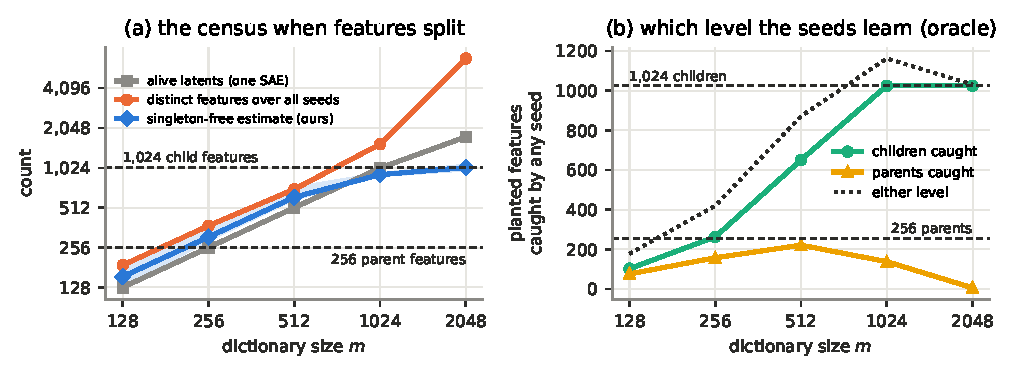
\includegraphics[width=\linewidth]{../figures/fig4_hierarchy.pdf}
\caption{\textbf{Features that split.} \HierParents{} planted parents, each with \HierC{} children (\HierChildren{} in all). (a) Counts against dictionary size, averaged over \HierDraws{} data draws; bands show the range over draws, and for the census the bootstrap intervals of both. The census rises with the dictionary and levels off at the child count only once there is room for every child. (b) Planted features caught by at least one of \SynSeeds{} seeds under oracle matching. Small dictionaries learn a mixture of parents and children.}
\label{fig:hier}
\end{figure}

\paragraph{Small dictionaries do not settle on the coarse level.} At $m=N/4$ there is room for exactly the \HierParents{} parents. Even so, the seeds learn a mixture: under oracle matching, \HierKidsQuarter{} children and \HierParsQuarter{} parents are caught by at least one seed. The census does not stop at \HierParents{}. It rises with the dictionary (\HierSfEighth, \HierSfQuarter{} and \HierSfHalf{} at $m=N/8$, $N/4$ and $N/2$), at \HierSfReachMed{} of the features reachable at either level (median; range \HierSfReachMin--\HierSfReachMax). A coarse level therefore does not create a false plateau.

\paragraph{Once the finest level fits, the census finds it.} At $m=2N$ the estimate is \HierSfDouble{} against \HierChildren{} children. It is within \HierSfErrDouble{} of the child count in both draws and at all three matching thresholds. Over the same seeds, the number of distinct latents reaches \HierUnionDouble{} (\HierUnionRatioMax-fold). For $m\ge N$, a median \HierJunkSingle{} of the features caught by only one seed match no planted feature at either level.

\paragraph{At $m=N$ the census undercounts.} The estimate is \HierSfFull{}, \HierSfErrFull{} below the child count, even though every child is caught by some seed. A likely cause is that the seeds disagree about the level: \HierParsFull{} parents are also caught by at least one seed. A child that only some seeds resolve looks rarer than it is. This setting is also the most sensitive to the threshold (\HierSfFullTauLo{} at $\tau=\TauLo$, \HierSfFullTauHi{} at $\tau=\TauHi$). At $\tau=\TauLo$ a parent latent can match a child latent, since their cosine of \HierParentCos{} clears the threshold. Held-out prediction is also worse with hierarchy. Fitted on four seeds, the singleton-free model overshoots the eight-seed count by a median of \HeldHierSmallSfMed{} for $m<N$ and \HeldHierBigSfMed{} (maximum \HeldHierBigSfMax) for $m\ge N$. ``No growth'' misses by \HeldHierSmallNoGrowthMed{} and \HeldHierBigNoGrowthMed{}.

Splitting changes how a census curve should be read, not whether the census works. At a given dictionary size, the census counts the features that size resolves, and a plateau marks the finest level the dictionaries can hold. On Pythia-70M the count keeps growing (\S\ref{sec:real}). Splitting produces the same growth whenever the finest level does not yet fit, so that growth alone does not show a fixed population larger than the dictionaries we trained.
